 
% !TEX TS-program = LuaLaTeX

%% Copyright (c) 2021 CuriousTorvald.

\documentclass[10pt, stock, openany, chapter]{memoir}


\usepackage{fontspec}
\setmainfont[Ligatures=TeX]{TeX Gyre Heros}
\newfontfamily\condensedfont{TeX Gyre Heros Cn}
\newfontfamily\titlefont{TeX Gyre Schola}
\newfontfamily\monofont[Ligatures={NoCommon, NoDiscretionary, NoHistoric, NoRequired, NoContextual}]{TeX Gyre Cursor}


\usepackage{fapapersize}
\usefapapersize{148mm,210mm,15mm,15mm,20mm,15mm} % A5 paper
\usepackage{afterpage}
\usepackage{hyperref}
\usepackage{graphicx}
\usepackage{tabulary}
\usepackage{longtable}
\usepackage[table]{xcolor}
\usepackage{ltablex}
\usepackage{parskip}
\usepackage{multicol}
\usepackage{soul}
\usepackage{verbatim}
\usepackage{etoolbox}
\usepackage[most]{tcolorbox}
\usepackage{listings}
\usepackage{amsmath,amssymb}
\usepackage{calc}
\usepackage{ifthen}
\usepackage[pdf]{graphviz}
\usepackage{caption}
\usepackage{subcaption}
\usepackage{makeidx}
\usepackage{multirow}
\usepackage{textcomp}
\usepackage{makecell}
\usepackage{anyfontsize}
\usepackage{cancel}
\usepackage{outlines}
\usepackage{lineno} % debug


\renewcommand\theadalign{bc}

\makeatletter
\newlength{\mytextsize}
\setlength{\mytextsize}{\f@size pt}
\newlength{\mybaselineskip}
\setlength{\mybaselineskip}{1.3\mytextsize}
\patchcmd{\verbatim@input}{\@verbatim}{\scriptsize\@verbatim}{}{}
\makeatother
\setlength{\baselineskip}{\mybaselineskip}

\frenchspacing
\setlength{\parindent}{0pt}
\setlength{\parskip}{\mytextsize}
\setsecnumdepth{subsection}

%% More compact itemize %%
\newenvironment{itemlist}{\vspace{0pt}\itemize}{\enditemize}

%% Idioms %%
\hyphenation{Java-script}
\hyphenation{ECMA-script}
\hyphenation{name-space}

\newcommand\forceindent{\hskip1.5em}

%% BASIC operators %%
\newcommand\tildechar{{\large\raisebox{-0.22ex}{\char`\~}}}
\newcommand{\instbit}[1]{\mbox{\scriptsize #1}}
\newcommand{\instbitrange}[2]{~\instbit{#1} \hfill \instbit{#2}~}


% Title styling
% \pretitle{\begin{flushright}}
% \posttitle{\par\end{flushright}}
% \preauthor{\begin{flushright}}
% \postauthor{\par\end{flushright}}

% new sections are new page
%\let\oldsection\chapter
%\renewcommand\chapter{\clearpage\oldsection}

% shorten spaces before section header
\setbeforesubsecskip{\mytextsize}
\setbeforesubsubsecskip{\mytextsize}

% extra space for table
\setlength{\extrarowheight}{0.166ex}

% chapter title -- no now page after
\renewcommand\chapterheadstart{} % kill the drop
\renewcommand\afterchapternum{\vskip 0.5em} % space between number and title
\setlength{\afterchapskip}{\baselineskip} % reduce space after chapter title
\makeatletter
\renewcommand\memendofchapterhook{%
\m@mindentafterchapter\@afterheading}
\makeatother


\definecolor{lgrey}{HTML}{eeeeee}
\sethlcolor{lgrey}
\renewcommand{\thefootnote}{\fnsymbol{footnote}}
\newcommand{\code}[1]{{\monofont\hl{\,#1\,}}}
\newcommand{\codebf}[1]{{\monofont \textbf{\hl{\,#1\,}}}}
%%\newcommand{\codeline}[1]{{\monofont\hl{\,#1\,}}}
\newcommand{\codeline}[1]{%
\colorbox{lgrey}{%
\begin{tabular*}{\textwidth}{l}%
\monofont #1 \\% TODO fill the cell with \hl colour
\end{tabular*}%
}}

\newtcolorbox{lgreybox}[1][]{%
  breakable,
  enhanced,
  colback=lgrey,
  attach title to upper,
  fontupper=\monofont,
  #1
}

\definecolor{sourcecomment}{HTML}{888888}

\lstset{frame=tb,
  language=Java,
  aboveskip=3mm,
  belowskip=3mm,
  showstringspaces=false,
  columns=flexible,
  basicstyle={\small\ttfamily},
  numbers=none,
  numberstyle=\textbf,
  keywordstyle=,
  commentstyle=\color{sourcecomment},
  stringstyle=\textbf,
  breaklines=true,
  breakatwhitespace=true,
  tabsize=3
}

\newcommand{\cnttoenglish}[2]{{%
\ifthenelse{#1=1}{one}{%
\ifthenelse{#1=2}{two}{%
\ifthenelse{#1=3}{three}{%
\ifthenelse{#1=4}{four}{%
\ifthenelse{#1=5}{five}{%
\ifthenelse{#1=6}{six}{%
\ifthenelse{#1=7}{seven}{%
\ifthenelse{#1=8}{eight}{%
\ifthenelse{#1=9}{nine}{%
\ifthenelse{#1=10}{ten}{%
\ifthenelse{#1=11}{eleven}{%
\ifthenelse{#1=12}{twelve}{%
\arabic{#1}%
}}}}}}}}}}}}} \ifthenelse{#1=1}{#2}{#2s}}

\addtocontents{toc}{\protect\thispagestyle{empty}} % no page number for the TOC header page
\aliaspagestyle{part}{empty} % aliasing PART as empty so that page number would not be printed
\aliaspagestyle{chapter}{section} % aliasing CHAPTER as section so that page numbering style would be the same as section


% The title
\newcommand{\thismachine}{TSVM}
\newcommand{\thedos}{TVDOS}
\newcommand{\tsvmver}{1.2}
\newcommand{\theedition}{Zeroth Edition}
\newcommand{\thepublishingdate}{0000-00-00}
\newcommand{\oreallypress}{\begingroup\hspace{0.083em}\large\textbf{O'REALLY\raisebox{1ex}{\scriptsize ?}} \large Press\endgroup}

\title{\vskip56pt 
\includegraphics[width=0.555\textwidth]{tsvmlogo_large} \vskip3pt \titlefont\Huge\textbf{PROGRAMMING GUIDE} \\ \Large \vspace{1.2em} For Version \tsvmver\hspace{0.75em}|\hspace{0.75em}\theedition}
\date{}
\author{}
\hypersetup{
	pdfauthor={CuriousTorvald},
	pdftitle={\thismachine\ Programming Guide for Version \tsvmver, \theedition},
	unicode=true,
	pdfcreator=\oreallypress
}

\makeindex
\begin{document}

\maketitle{}
\thispagestyle{empty}
\vfill
\oreallypress

\newpage

\chapter*{\ }

\copyright\ 2021-- \ Minjae Song (``CuriousTorvald'')

Copyrighted under the terms of MIT License

\oreallypress, Cyberworld

\quad\\

\begin{center}
\begin{tabulary}{\textwidth}{ll}
Zeroth Edition (for version 1.0): & \thepublishingdate
\end{tabulary}
\end{center}

\thispagestyle{empty}

\newpage

\setcounter{page}{3}
\tableofcontents*


%\linenumbers % debug

\openright
\chapter{Introduction}
\tbas{} is a BASIC dialect and its interpreter. \tbas emulates most of the common BASIC syntax while adds more advanced and up-to-date concepts gracefully, such as user-defined function that can \emph{actually} recurse, arbitrary list construction using CONS-operator and some of the features on functional programming such as \code{MAP} and \code{FOLD}.

This is the documentation for \tbas{} \tbasver{}.

\small\emph{Henceforward this documentation will use more friendly and sometimes vulgar language because that's more fun to write!}

\openany

% \chapter{Version Changes}

\input{changes1.2}
\input{changes1.1}


\part{The Virtual Machine}

\chapter{Virtual Machine}
\chapter{\thismachine}

\section{Specs}

\begin{outline}
\1 16 MB memory space with maximum 8 MB of scratchpad memory
\1 7 peripheral card slots, each can map 1 MB of memory to the memory space
\1 Standard graphics adapter on slot 1, with 256 simultaneous colours, 560\times448 pixels framebuffer and 80-column 32-row text buffer
\1 Built-in mouse input support
\1 4 serial ports to connect disk drives, modems and other computers
\end{outline}

There are three memories on the system: Hardware Memory (8 MB), Scratchpad Memory (up to 8 MB) and Program Memory (infinite!)

Your Javascript program is stored into the Program Memory, and since its capacity is limitless, you can put a large graphics directly into your Javascript source code, but the Program Memory is the slowest of all three memories. For faster graphics, you need to store them onto the Scratchpad Memory then DMA-Copy them to the graphics adapter.

\section{Javascript Extensions}

\index{js extensions}\thismachine\ provides the extra functions for your convenience.

\begin{outline}
\1\inlinesynopsis[Array]{head}[]{returns the first element of the array.}
\1\inlinesynopsis[Array]{last}[]{returns the last element of the array.}
\1\inlinesynopsis[Array]{tail}[]{returns the subarray that omits the \emph{head} element.}
\1\inlinesynopsis[Array]{init}[]{returns the subarray that omits the \emph{last} element.}
\1\inlinesynopsis[Array]{sum}[selector]{returns the sum of the elements of the array. Selector is optionally defined to indicate how the value must be transformed to obtain the sum.}
\1\inlinesynopsis[Array]{max}[selector]{returns the maximum among the elements of the array. Selector is optionally defined to indicate how the value must be transformed to obtain the max.}
\1\inlinesynopsis[String]{head}[]{returns the first character of the string.}
\1\inlinesynopsis[String]{last}[]{returns the last character of the string.}
\1\inlinesynopsis[String]{tail}[]{returns the substring that omits the \emph{head} character.}
\1\inlinesynopsis[String]{init}[]{returns the substring that omits the \emph{last} character.}
\1\inlinesynopsis[String]{trimNull}[]{trims null characters at the \emph{end} of the string.}
\end{outline}



\chapter{Libraries}



\section{Standard Input and Output}

\index{stdio (library)}These are standard input/output functions:

\begin{outline}
\1\inlinesynopsis{print}[String]{prints a string without a new line.}
\1\inlinesynopsis{println}[String]{prints a string with a new line.}
\1\inlinesynopsis{printerr}[String]{prints a string to error output without a new line.}
\1\inlinesynopsis{printerrln}[String]{prints a string to error output with a new line.}
\1\inlinesynopsis{read}[]{reads a string from the keyboard. Hit the Return to finish reading.}
\end{outline}

\section{Console}

\index{console (library)}Console library contains the functions for screen text manipulation.

\namespaceis{Console}{con}

Properties:
\begin{outline}
\1\inlinesynopsis{KEY\_HOME}{A keycode for the Home key. 199}
\1\inlinesynopsis{KEY\_UP}{A keycode for the Up arrow key. 200}
\1\inlinesynopsis{KEY\_PAGE\_UP}{A keycode for the Page Up key. 201}
\1\inlinesynopsis{KEY\_LEFT}{A keycode for the Left arrow key. 203}
\1\inlinesynopsis{KEY\_RIGHT}{A keycode for the Right arrow key. 205}
\1\inlinesynopsis{KEY\_END}{A keycode for the End key. 207}
\1\inlinesynopsis{KEY\_DOWN}{A keycode for the Down arrow key. 208}
\1\inlinesynopsis{KEY\_PAGE\_DOWN}{A keycode for the Page Down key. 209}
\1\inlinesynopsis{KEY\_INSERT}{A keycode for the Insert key. 210}
\1\inlinesynopsis{KEY\_DELETE}{A keycode for the Delete key. 211}
\1\inlinesynopsis{KEY\_BACKSPACE}{A keycode for the Backspace key. 8}
\1\inlinesynopsis{KEY\_TAB}{A keycode for the Tab key. 9}
\1\inlinesynopsis{KEY\_RETURN}{A keycode for the Return key. 10}
\end{outline}

Functions:
\begin{outline}
\1\formalsynopsis{getch}{}{Returns a key code read from the keyboard.}
\1\formalsynopsis{poll\_keys}{}[IntArray(8) of Keycodes]{Poll the keyboard, then returns the captured keycodes. If less than 8 keys were held down at the moment of the polling, 0 will be substituted for the spot on the array.}
\1\formalsynopsis{move}{y: Int, x: Int}{Moves the text cursor to the given position. Note that the cursor position starts at 1.}
\1\formalsynopsis{addch}{char: Int}{Puts a character denoted by its code point to where the text cursor is. The cursor will not advance. NOTE: this function accesses the graphics device directly, which may not be desirable; use \code{prnch} when you really need to \code{print} the character.}
\1\formalsynopsis{mvaddch}{y: Int, x: Int, char: Int}{Combination of \code{move} and \code{addch}.}
\1\formalsynopsis{prnch}{char: Int}{Prints out a character denoted by its code point using the escape sequences. Unlike \code{addch} this function actually print out a character, which makes difference in certain situation.}

\1\formalsynopsis{getmaxyx}{}[IntArray(2)]{Returns the size of the terminal in row-column order.}
\1\formalsynopsis{getyx}{}[IntArray(2)]{Returns the current position of the text cursor in row-column order.}
\1\formalsynopsis{curs\_up}{}{Moves the text cursor up once.}
\1\formalsynopsis{curs\_down}{}{Moves the text cursor down once. Screen will scroll if the cursor moves out of the screen.}
\1\formalsynopsis{curs\_left}{}{Moves the text cursor left once.}
\1\formalsynopsis{curs\_right}{}{Moves the text cursor right once. Will wrap to the next line if the cursor moves out of the screen.}
\1\formalsynopsis{curs\_set}{mode: Int}{Hides or shows the text cursor. 0 to hide, nonzero to show.}
\1\formalsynopsis{hitterminate}{}[Boolean]{Polls the keyboard and returns true if the Ctrl-C combination were held down.}
\1\formalsynopsis{hiteof}{}[Boolean]{Polls the keyboard and returns true if the Ctrl-D combination were held down.}
\1\formalsynopsis{resetkeybuf}{}{Zero-fills the keyboard input buffer.}
\1\formalsynopsis{video\_reverse}{}{Swaps the foreground and background colour of the text.}
\1\formalsynopsis{color\_fore}{code: Int}{Defines the foreground colour of the text. 0 -- black, 1 -- red, 2 -- green, 3 -- yellow, 4 -- blue, 5 -- magenta, 6 -- cyan, 7 -- white, -1 -- transparent}
\1\formalsynopsis{color\_back}{code: Int}{Defines the background colour of the text.}
\1\formalsynopsis{color\_pair}{fore: Int, back: Int}{Defines the foreground and background colour of the text. Colour code for this function differs from the \code{color\_back} and \code{color\_fore}; please refer to the \ref{colourpalette}.}
\1\formalsynopsis{clear}{}{Clears the text buffer. The framebuffer (if any) will not be affected.}
\1\formalsynopsis{reset\_graphics}{}{Resets foreground and background colour to defaults and makes the cursor visible if it was hidden.}
\end{outline}



\section{Gzip}

\index{gzip (library)}Gzip allows texts and bytes and compressed and decompressed using the gzip format.

\namespaceis{Gzip}{gzip}

\begin{outline}
\1\formalsynopsis{comp}{String}[Uint8Array]{Compresses the given string.}
\1\formalsynopsis{comp}{Uint8Array}[Uint8Array]{Compresses the given bytes.}
\1\formalsynopsis{compTo}{str: String, outputptr: Int}[Int]{Compresses the given string onto the memory, then returns the size of the compressed bytes.}
\1\formalsynopsis{compTo}{bytes: Uint8Array, outputptr: Int}[Int]{Compresses the given bytes onto the memory, then returns the size of the compressed bytes.}
\1\formalsynopsis{compFromTo}{inputptr: Int, length: Int, outputptr: Int}[Int]{Compresses the bytes onto the memory, then returns the size of the compressed bytes.}
\1\formalsynopsis{decomp}{String}[Uint8Array]{Decompresses the given string (compressed bytes represented as series of characters)}
\1\formalsynopsis{decomp}{Uint8Array}[Uint8Array]{Decompresses the given bytes.}
\1\formalsynopsis{decompTo}{str: String, outputptr: Int}[Int]{Decompresses the given string onto the memory, then returns the size of the decompressed bytes.}
\1\formalsynopsis{decompTo}{bytes: Uint8Array, outputptr: Int}[Int]{Decompresses the given bytes onto the memory, then returns the size of the decompressed bytes.}
\1\formalsynopsis{decompFromTo}{inputptr: Int, length: Int, outputptr: Int}[Int]{Decompresses the bytes onto the memory, then returns the size of the decompressed bytes.}
\end{outline}



\section{Base64}

\index{base64 (library)}Base64 allows encoding of the binary data into the ASCII-strings and vice-versa.

\namespaceis{Base64}{base64}

\begin{outline}
\1\formalsynopsis{atob}{String}[Uint8Array]{Decodes the Base64 string to bytes.}
\1\formalsynopsis{atostr}{String}[String]{Decodes the Base64 string to string.}
\1\formalsynopsis{btoa}{Uint8Array}[String]{Encodes bytes to Base64 string.}
\end{outline}



\section{Sys}

Sys library allows programmers to manipulate the system in low-level.

\namespaceis{Sys}{sys}

\begin{outline}
\1\formalsynopsis{poke}{address: Int, value: Int}{Puts a value into the memory of the specified address.}
\1\formalsynopsis{peek}{address: Int}[Int]{Reads a value from the memory of the specified address.}
\1\formalsynopsis{malloc}{size: Int}[Int]{Allocates a space of the given size on the Scratchpad memory and returns its pointer (starting address)}
\1\formalsynopsis{free}{pointer: Int}{Frees the memory space previously \code{malloc}'d}
\1\formalsynopsis{memcpy}{from: Int, to: Int, length: Int}{Copies the memory block of the given length. From and To are pointers.}
\1\formalsynopsis{mapRom}{romSlotNum: Int}{Maps the contents on the given ROM to the memory address {-\nobreak65537.\nobreak.-\nobreak131072}}
\1\formalsynopsis{romReadAll}{}[String]{Reads the mapped ROM and returns its contents as a string.}
\1\formalsynopsis{uptime}{}[Long]{Returns the uptime of the system in miliseconds.}
\1\formalsynopsis{currentTimeInMills}{}[Long]{Returns the current time in miliseconds since the epoch (exact time varies by the system)}
\1\formalsynopsis{nanoTime}{}[Long]{Returns the current time in nanoseconds since the epoch (exact time varies by the system)}
\1\formalsynopsis{print}{Anything}{Prints the given value onto the printstream.}
\1\formalsynopsis{println}{Anything}{Prints the given value plus a newline onto the printstream.}
\1\formalsynopsis{readKey}{}[Int]{Reads a key press and returns its keycode. The program execution will be paused until a key is pressed.}
\1\formalsynopsis{read}{}[String]{Reads a text the user has typed and returns is as a string. The reading will be terminated when the user hits the Return key.}
\1\formalsynopsis{readNoEcho}{}[String]{Identical to \code{read} but the text the user is typing will not be printed to the screen.}
\1\formalsynopsis{spin}{}[]{Do nothing for 4 miliseconds. Always use this function for busy-waiting as the virtual machine will hang without one.}
\1\formalsynopsis{waitForMemChg}{address: Int, andMask: Int, xorMask: Int}[]{Do nothing until a memory value is changed. More specifically, this function will \code{spin} while:$$ (\mathrm{peek}(addr)\ \mathrm{xor}\ xorMask)\ \mathrm{and}\ andMask = 0 $$}
\1\formalsynopsis{getSysRq}{}[Boolean]{Returns true if System Request key is down.}
\1\formalsynopsis{unsetSysRq}{}{After using the System Request key, call this function to `release' the key so that other programs can use it.}
\1\formalsynopsis{maxmem}{}[Int]{returns the size of the Scratchpad Memory in bytes.}
\1\formalsynopsis{getUsedMem}{}[Int]{Returns how many memories can be \code{malloc}'d.}
\1\formalsynopsis{getMallocStatus}{}[IntArray(2)]{Returns the \code{malloc} status in following order:$$ [\mathrm{Malloc\ unit\ size,\ allocated\ block\ counts}] $$}
\end{outline}





\chapter{Serial Communication}

Some peripherals such as disk drives are connected through the ``Serial Communication''.

Unlike the name suggests, Serial Communication is not at all \emph{serial}; it's more like a \emph{block communication}.

\section{Concept of the Block Communication}

\index{block communication}As long as the Sender and the Receiver are somehow connected and being recognised, the communication channel between two devices are open and available. There are two blocks per port: the send-block and the receive-block, and the contents of the blocks are memory-mapped\footnote{Both blocks are mapped to the same port; writing to the address writes to the send-block while reading reads from the receive-block. Reading from write-block or writing to the read-block is not possible}. \emph{Write} writes the sender's send-block onto the receiver's receive-block while \emph{Read} pulls the message from the receiver's send-block and writes to the sender's receive-block.

When the read/write operation is being processed, each side emits ``busy'' flag indicating they are \emph{busy}. Sending/receiving data while one side is busy is considered as an undefined behaviour.


\section{The Com Library}

\index{com (library)}portNo is a number of the port in 0--3, 0 being the first port.

\namespaceis{Com}{com}

\begin{outline}
\1\formalsynopsis{sendMessage}{portNo: Int, message: String}{Sends message to the port and returns status code the other machine emits.}
\1\formalsynopsis{fetchResponse}{portNo: Int}[String]{Fetches the message composed by other device to this machine.}
\1\formalsynopsis{sendMessageGetBytes}{portNo: Int, message: String}[String]{Sends message, waits for responce, then returns the received message.}
\1\formalsynopsis{waitUntilReady}{portNo: Int}{Blocks the program until the other device is ready.}
\1\formalsynopsis{pullMessage}{portNo: Int}[String]{Make other device to initiate sending and returns the message receive from the other device.\\NOTE: this is not a function you're looking for it you're just getting the response after the sendMessage; use fetchResponse for that.}
\1\formalsynopsis{getStatusCode}{portNo: Int}[Int]{Returns the status code of the other device.}
\1\formalsynopsis{getDeviceStatus}{portNo: Int}[\{code: Int, message: String\}]{Returns the status message of the other device. Different types of devices may have different messages.}
\1\formalsynopsis{areYouThere}{portNo: Int}[Boolean]{Returns true if there is other device connected and is working.}
\end{outline}


\subsection{Code Example: Get a File from the Disk Drive}

\begin{lstlisting}
com.sendMessage(0, "DEVRST\x17")  // resets the disk drive
com.sendMessage(0, 'OPENR"my-awesome.txt",1')  // tells the disk drive to open a file named 'my-awesome.txt' from the drive number 1 for reading
let status = com.getStatusCode(0)
if (0 == status){
	com.sendMessage(0, "READ")  // tells the disk drive that I'm about to read the file just opened
	status = com.getStatusCode(0)
	if (0 == status) {
		println("Reading file...")
		let g = com.pullMessage(0)  // will negotiate with the disk drive and read the entire file
		println("Here's your file:")
		println(g)
	} else printerrln("I/O Error " + status)
} else printerrln("I/O Error " + status)
\end{lstlisting}


\subsection{Code Example: Write a Text to the Disk Drive}

\begin{lstlisting}
com.sendMessage(0, "DEVRST\x17")  // resets the disk drive
com.sendMessage(0, 'OPENW"my-awesomer.txt",1')  // tells the disk drive to open a file named 'my-awesomer.txt' from the drive number 1 for writing
let status = com.getStatusCode(0)
if (0 == status){
	com.sendMessage(0, "WRITE1234")  // tells the disk drive that I'm about to write to the file just opened. 1234 is a size of the text to write
	status = com.getStatusCode(0)
	if (0 == status) {
		println("Writing file...")
		com.sendMessage(0, myAwesomeText)  // myAwesomeText must be in the same length as what we have told to the disk drive
		com.sendMessage(0, "FLUSH")  // tells the disk drive to empty out whatever is left on its internal buffer, and puts the drive to ready-mode
		com.sendMessage(0, "CLOSE")  // tells the disk drive to close the file
	} else printerrln("I/O Error " + status)
} else printerrln("I/O Error " + status)
\end{lstlisting}



\section{Communication MMIO and How It Actually Works}

\index{MMIO-com}The status flags and transfer/receive blocks are memory-mapped to these address:
\footnote{RW stands for read-write status. RW means both reading and writing is posseble, RO means it's read-only}


\begin{tabulary}{\textwidth}{rcL}
Address & RW & Description \\
\hline
-4077..-4080 & RW & Status Code (-128--127) for Writing Port 1--4 \\
-4081..-4084 & RO & Status Code (-128--127) of the Receiver 1--4 \\
-4085..-4092 & RO & Transfer Status Bits for Port 1--4 (two bytes per port) \\
-4093..-4096 & RW & Transfer Control for Port 1--4 \\
-4097..-8192 & RW &   Message Block for Port 1 \\
-8193..-12288 & RW &  Message Block for Port 2 \\
-12289..-16384 & RW & Message Block for Port 3 \\
-16385..-20480 & RW & Message Block for Port 4
\end{tabulary}

\subsection{Transfer Status Bits and Transfer Control}

The com-port will behave differently if you're writing to or reading from the address. In other words, you cannot read what you have just wrote because the reading will put the port in a different state.

\begin{figure}[h]
\begin{center}
\setlength{\tabcolsep}{4pt}
\begin{tabular}{p{32mm}@{}p{12mm}@{}p{12mm}@{}p{16mm}@{}p{24mm}l}
\\
\instbitrange{7}{0} &
\multicolumn{1}{c}{\instbit{15}} &
\instbitrange{14}{12} &
\instbitrange{11}{8} \\
\cline{1-4}
\multicolumn{1}{|c}{size-LSB} &
\multicolumn{1}{||c|}{read} &
\multicolumn{1}{c|}{000} &
\multicolumn{1}{c|}{size-MSB} &
\ Status Bits \\
\cline{1-4}

\end{tabular}
\begin{tabular}{p{10mm}@{}p{20mm}@{}p{16mm}@{}p{16mm}@{}p{16mm}@{}p{20mm}@{}p{24mm}l}
\\
\instbitrange{7}{6} &
\instbitrange{5}{4} &
\multicolumn{1}{c}{\instbit{3}} &
\multicolumn{1}{c}{\instbit{2}} &
\multicolumn{1}{c}{\instbit{1}} &
\multicolumn{1}{c}{\instbit{0}} & \\
\cline{1-6}
\multicolumn{1}{|c|}{00} &
\multicolumn{1}{c|}{M/S} &
\multicolumn{1}{c|}{T/R} &
\multicolumn{1}{c|}{busy} &
\multicolumn{1}{c|}{ready} &
\multicolumn{1}{c|}{hello} &
\ Control Bits \\
\cline{1-6}

\end{tabular}
\end{center}
\caption{Transfer Status and Transfer Control Bits}
\label{fig:transfer-status-bits}
\end{figure}

\begin{outline}
\1\inlinesynopsis{size-LSB/MSB}{size of the data within the block}
 \2\argsynopsis{read}{from the other device}
 \2\argsynopsis{write}{what the device is about to send. size of zero must be interpreted as 4096}
\1\inlinesynopsis{read}{bit is set if the other device \emph{hasNext}, unset otherwise or the device is not present}
\1\inlinesynopsis{M/S}{Master/Slave setup of the other device. Typically a disk drive is slave-only (01), a computer is both (11)}
\1\inlinesynopsis{T/R}{Send-Receive mode for the port. Set the bit to send from the port, unset to read}
\1\inlinesynopsis{busy}{device busy/transfer trigger}
 \2\argsynopsis{read}{the port is receiving something if the bit is set}
 \2\argsynopsis{write}{setting this bit initiates transfer. If the T/R bit is set, the device will send the message out, otherwise the other device will start the transfer}
\1\inlinesynopsis{ready}{write to indicate this device is ready to receive; read to know if the other device is ready}
\1\inlinesynopsis{hello}{bit is set if the other device is connected}
\end{outline}



\chapter{Human Interface}


\section{Keyboard}

TODO

\subsection{Keycodes}

\index{keycodes}This is a table of keycodes recognised by the LibGDX, a framework that \thismachine\ runs on.

\begin{longtable}{*{2}{m{\textwidth}}}\hline
\endfirsthead
\endhead

\endfoot
\hline
\endlastfoot
\centering
\begin{tabulary}{\textwidth}{rl}
Key & Code \\
\hline
\ttfamily{0} & 7 \\
\ttfamily{1} & 8 \\
\ttfamily{2} & 9 \\
\ttfamily{3} & 10 \\
\ttfamily{4} & 11 \\
\ttfamily{5} & 12 \\
\ttfamily{6} & 13 \\
\ttfamily{7} & 14 \\
\ttfamily{8} & 15 \\
\ttfamily{9} & 16 \\
$\hookleftarrow$ & 66 \\
\condensedfont{BkSp} & 67 \\
\condensedfont{Tab} & 61 \\
\ttfamily{`} & 68 \\
\ttfamily{'} & 75 \\
\ttfamily{;} & 43 \\
\ttfamily{,} & 55 \\
\ttfamily{.} & 56 \\
\ttfamily{/} & 76 \\
\ttfamily{[}\hspace*{0.083em} & 71 \\
\ttfamily{]}\hspace*{-0.083em} & 72 \\
\ttfamily{-} & 69 \\
\end{tabulary}
\begin{tabulary}{\textwidth}{rl}
Key & Code \\
\hline
\ttfamily{+} & 70 \\
\ttfamily{A} & 29 \\
\ttfamily{B} & 30 \\
\ttfamily{C} & 31 \\
\ttfamily{D} & 32\\
\ttfamily{E} & 33 \\
\ttfamily{F} & 34 \\
\ttfamily{G} & 35 \\
\ttfamily{H} & 36 \\
\ttfamily{I} & 37 \\
\ttfamily{J} & 38 \\
\ttfamily{K} & 39 \\
\ttfamily{L} & 40 \\
\ttfamily{M} & 41 \\
\ttfamily{N} & 42 \\
\ttfamily{O} & 43 \\
\ttfamily{P} & 44 \\
\ttfamily{Q} & 45 \\
\ttfamily{R} & 46 \\
\ttfamily{S} & 47 \\
\ttfamily{T} & 48 \\
\ttfamily{U} & 49 \\
\end{tabulary}
\begin{tabulary}{\textwidth}{rl}
Key & Code \\
\hline
\ttfamily{V} & 50 \\
\ttfamily{W} & 51 \\
\ttfamily{X} & 52 \\
\ttfamily{Y} & 53 \\
\ttfamily{Z} & 54 \\
\condensedfont{LCtrl} & 57 \\
\condensedfont{RCtrl} & 58 \\
\condensedfont{LShift} & 59 \\
\condensedfont{RShift} & 60 \\
\condensedfont{LAlt} & 129 \\
\condensedfont{RAlt} & 130 \\
$\uparrow$ & 19 \\
$\downarrow$ & 20 \\
$\leftarrow$ & 21 \\
$\rightarrow$ & 22 \\
\condensedfont{Ins} & 133 \\
\condensedfont{Del} & 112 \\
\condensedfont{PgUp} & 92 \\
\condensedfont{PgDn} & 93 \\
\condensedfont{Home} & 3 \\
\condensedfont{End} & 123 \\
F1 & 131 \\
\end{tabulary}
\begin{tabulary}{\textwidth}{rl}
Key & Code \\
\hline
F2 & 132 \\
F3 & 133 \\
F4 & 134 \\
F5 & 135 \\
F6 & 136 \\
F7 & 137 \\
F8 & 138 \\
F9 & 139 \\
F10 & 140 \\
F11 & 141 \\
F12 & 142 \\
\condensedfont{Num} \ttfamily{0} & 144 \\
\condensedfont{Num} \ttfamily{1} & 145 \\
\condensedfont{Num} \ttfamily{2} & 146 \\
\condensedfont{Num} \ttfamily{3} & 147 \\
\condensedfont{Num} \ttfamily{4} & 148 \\
\condensedfont{Num} \ttfamily{5} & 149 \\
\condensedfont{Num} \ttfamily{6} & 150 \\
\condensedfont{Num} \ttfamily{7} & 151 \\
\condensedfont{Num} \ttfamily{8} & 152 \\
\condensedfont{Num} \ttfamily{9} & 153 \\
\condensedfont{NumLk} & 78 \\
\end{tabulary}
\end{longtable}


\section{Mouse}

TODO


\chapter{Peripherals and Memory Mapping}

\index{memory map}The hardware registers and memories of a peripheral is memory-mapped to the specific addresses that can be \code{peek}ed and \code{poke}d.

The memory map of \thismachine\ is illustrated as following:

\newcommand{\memend}[1]{\raisebox{1.3em}{#1}}
\newcommand{\memlabel}[1]{\raisebox{-0.1ex}{#1}}

\begin{tikzpicture}
\centering
\draw[thick] (0,0) rectangle (6, 12);
% Memory starting addr
\draw (6,12) node[anchor=north west] {8388607};
\draw[thick] (0,8) node[anchor=north east] {-1} -- (6,8);
\draw (0,7) node[anchor=north east] {-1048577} -- (6,7);
\draw (0,6) node[anchor=north east] {-2097153} -- (6,6);
\draw (0,5) node[anchor=north east] {-3145729} -- (6,5);
\draw (0,4) node[anchor=north east] {-4194305} -- (6,4);
\draw (0,3) node[anchor=north east] {-5242881} -- (6,3);
\draw (0,2) node[anchor=north east] {-6291457} -- (6,2);
\draw (0,1) node[anchor=north east] {-7340033} -- (6,1);
% Memory ending addr
\draw (0,8) node[anchor=east] {\memend{0}};
\draw (6,7) node[anchor=west] {\memend{-1048576}};
\draw (6,6) node[anchor=west] {\memend{-2097152}};
\draw (6,5) node[anchor=west] {\memend{-3145728}};
\draw (6,4) node[anchor=west] {\memend{-4194304}};
\draw (6,3) node[anchor=west] {\memend{-5242880}};
\draw (6,2) node[anchor=west] {\memend{-6291456}};
\draw (6,1) node[anchor=west] {\memend{-7340032}};
\draw (6,0) node[anchor=west] {\memend{-8388608}};
% Labels
\draw(0,12.5) node[anchor=north east] {Start};
\draw(6,12.5) node[anchor=north west] {End};

\draw(3,10)  node[anchor=mid] {\memlabel{Scratchpad Memory}};
\draw(3,7.5) node[anchor=mid] {\memlabel{MMIO Area}};
\draw(3,6.5) node[anchor=mid] {\memlabel{Peripheral Memory \#1}};
\draw(3,5.5) node[anchor=mid] {\memlabel{Peripheral Memory \#2}};
\draw(3,4.5) node[anchor=mid] {\memlabel{Peripheral Memory \#3}};
\draw(3,3.5) node[anchor=mid] {\memlabel{Peripheral Memory \#4}};
\draw(3,2.5) node[anchor=mid] {\memlabel{Peripheral Memory \#5}};
\draw(3,1.5) node[anchor=mid] {\memlabel{Peripheral Memory \#6}};
\draw(3,0.5) node[anchor=mid] {\memlabel{Peripheral Memory \#7}};
\end{tikzpicture}

The MMIO Area is further divided as shown:

\begin{tikzpicture}
\centering
\draw[thick] (0,0) rectangle (6, 8);
% Memory starting addr
\draw (0,8) node[anchor=north east] {-1} -- (6,8);
\draw (0,7) node[anchor=north east] {-131073} -- (6,7);
\draw (0,6) node[anchor=north east] {-262145} -- (6,6);
\draw (0,5) node[anchor=north east] {-393217} -- (6,5);
\draw (0,4) node[anchor=north east] {-524289} -- (6,4);
\draw (0,3) node[anchor=north east] {-655361} -- (6,3);
\draw (0,2) node[anchor=north east] {-786433} -- (6,2);
\draw (0,1) node[anchor=north east] {-917505} -- (6,1);
% Memory ending addr
\draw (6,7) node[anchor=west] {\memend{-131072}};
\draw (6,6) node[anchor=west] {\memend{-262144}};
\draw (6,5) node[anchor=west] {\memend{-393216}};
\draw (6,4) node[anchor=west] {\memend{-524288}};
\draw (6,3) node[anchor=west] {\memend{-655360}};
\draw (6,2) node[anchor=west] {\memend{-786432}};
\draw (6,1) node[anchor=west] {\memend{-917504}};
\draw (6,0) node[anchor=west] {\memend{-1048576}};
% Labels
\draw(0,8.5) node[anchor=north east] {Start};
\draw(6,8.5) node[anchor=north west] {End};

\draw(3,7.5) node[anchor=mid] {\memlabel{MMIO for Main Hardwares}};
\draw(3,6.5) node[anchor=mid] {\memlabel{MMIO for Peripheral \#1}};
\draw(3,5.5) node[anchor=mid] {\memlabel{MMIO for Peripheral \#2}};
\draw(3,4.5) node[anchor=mid] {\memlabel{MMIO for Peripheral \#3}};
\draw(3,3.5) node[anchor=mid] {\memlabel{MMIO for Peripheral \#4}};
\draw(3,2.5) node[anchor=mid] {\memlabel{MMIO for Peripheral \#5}};
\draw(3,1.5) node[anchor=mid] {\memlabel{MMIO for Peripheral \#6}};
\draw(3,0.5) node[anchor=mid] {\memlabel{MMIO for Peripheral \#7}};
\end{tikzpicture}

\chapter{Text and Graphics Display}

TODO: Textbuf, pixelbuf, graphics mode, chart of the draw order

\section{Text Buffer}

\index{text buffer}The reference text buffer stores 80 columns, 32 rows of characters with separate foreground and each character has separate 256 foreground and background colours.

While the graphics adapters can be plugged into any peripheral slot, it is highly recommended they occupy the 1st slot.

Text buffer is memory-mapped to the following address offset:

\subsection{Code Page}
\label{codepage}

\index{code page}By default \thismachine\ uses slightly modified version of CP-437, this is a character map of it:

{\centering
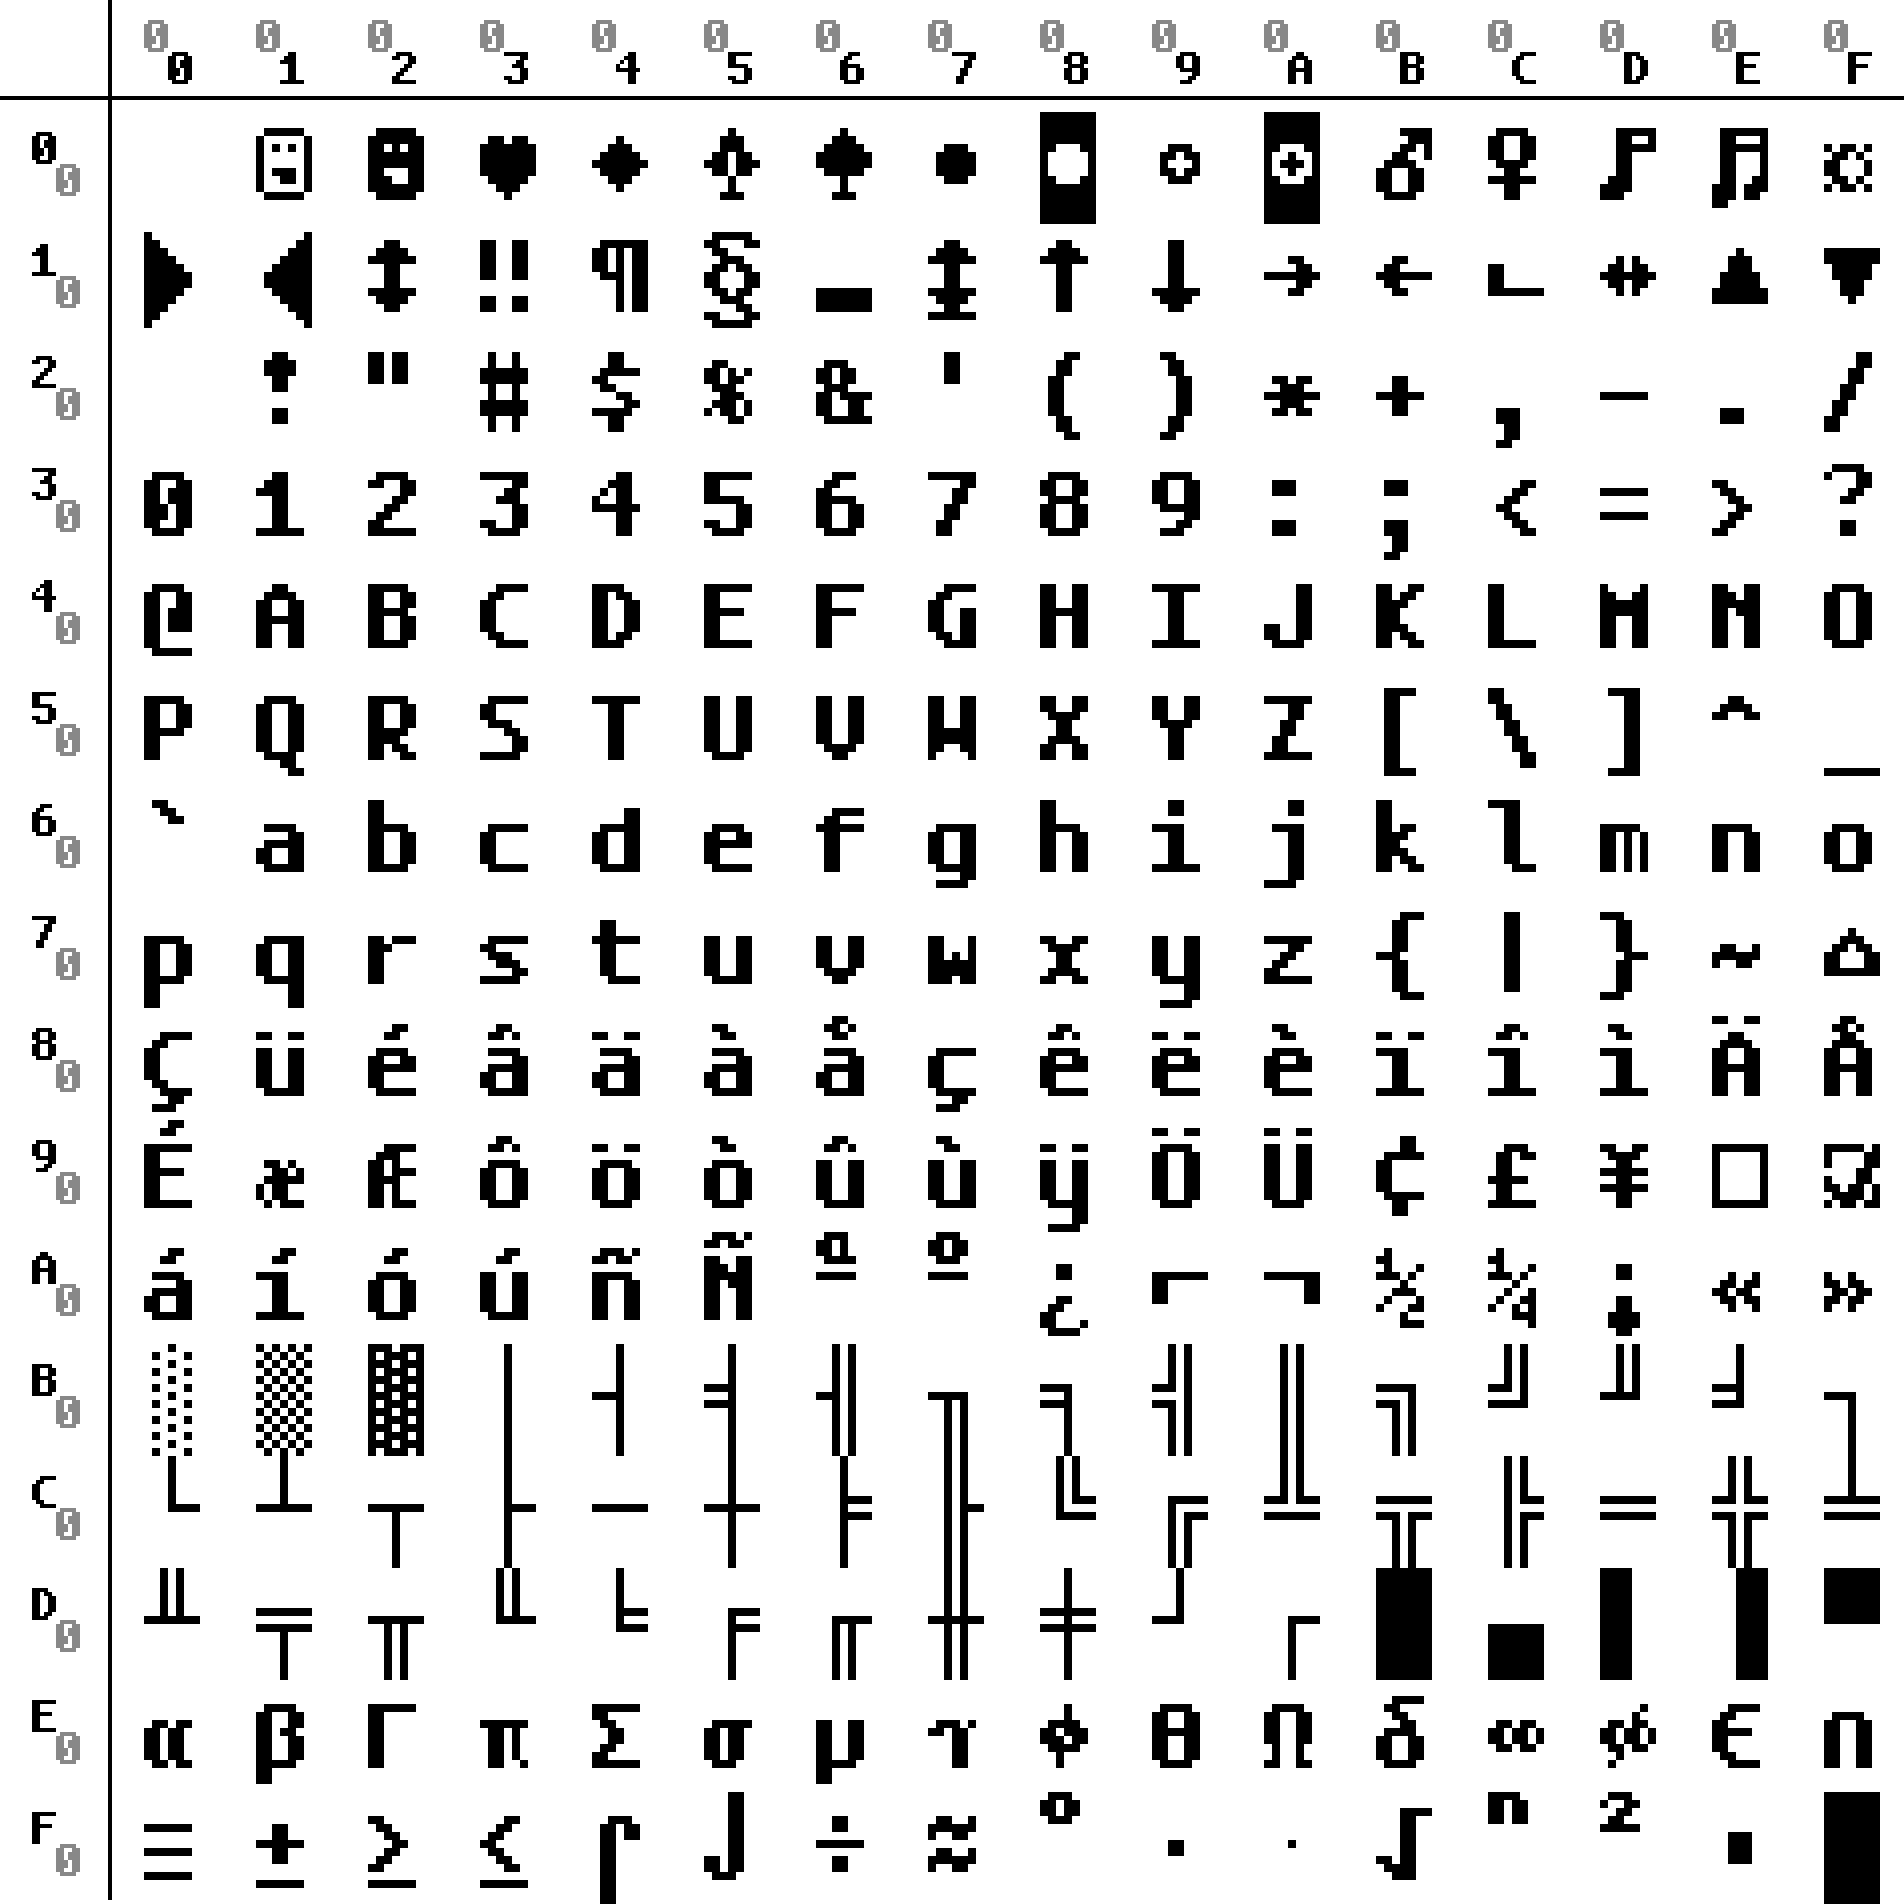
\includegraphics[width=\linewidth]{tsvmcp.png}
\captionof{figure}{\thismachine\ Character Map}
\label{fig:codepage}
}
\newpage


\section{Frame Buffer}

TODO

\subsection{Colour Palette}
\label{colourpalette}

\index{colour palette}By default the reference graphics adapter of the \thismachine\ uses following colour palette:

{\centering
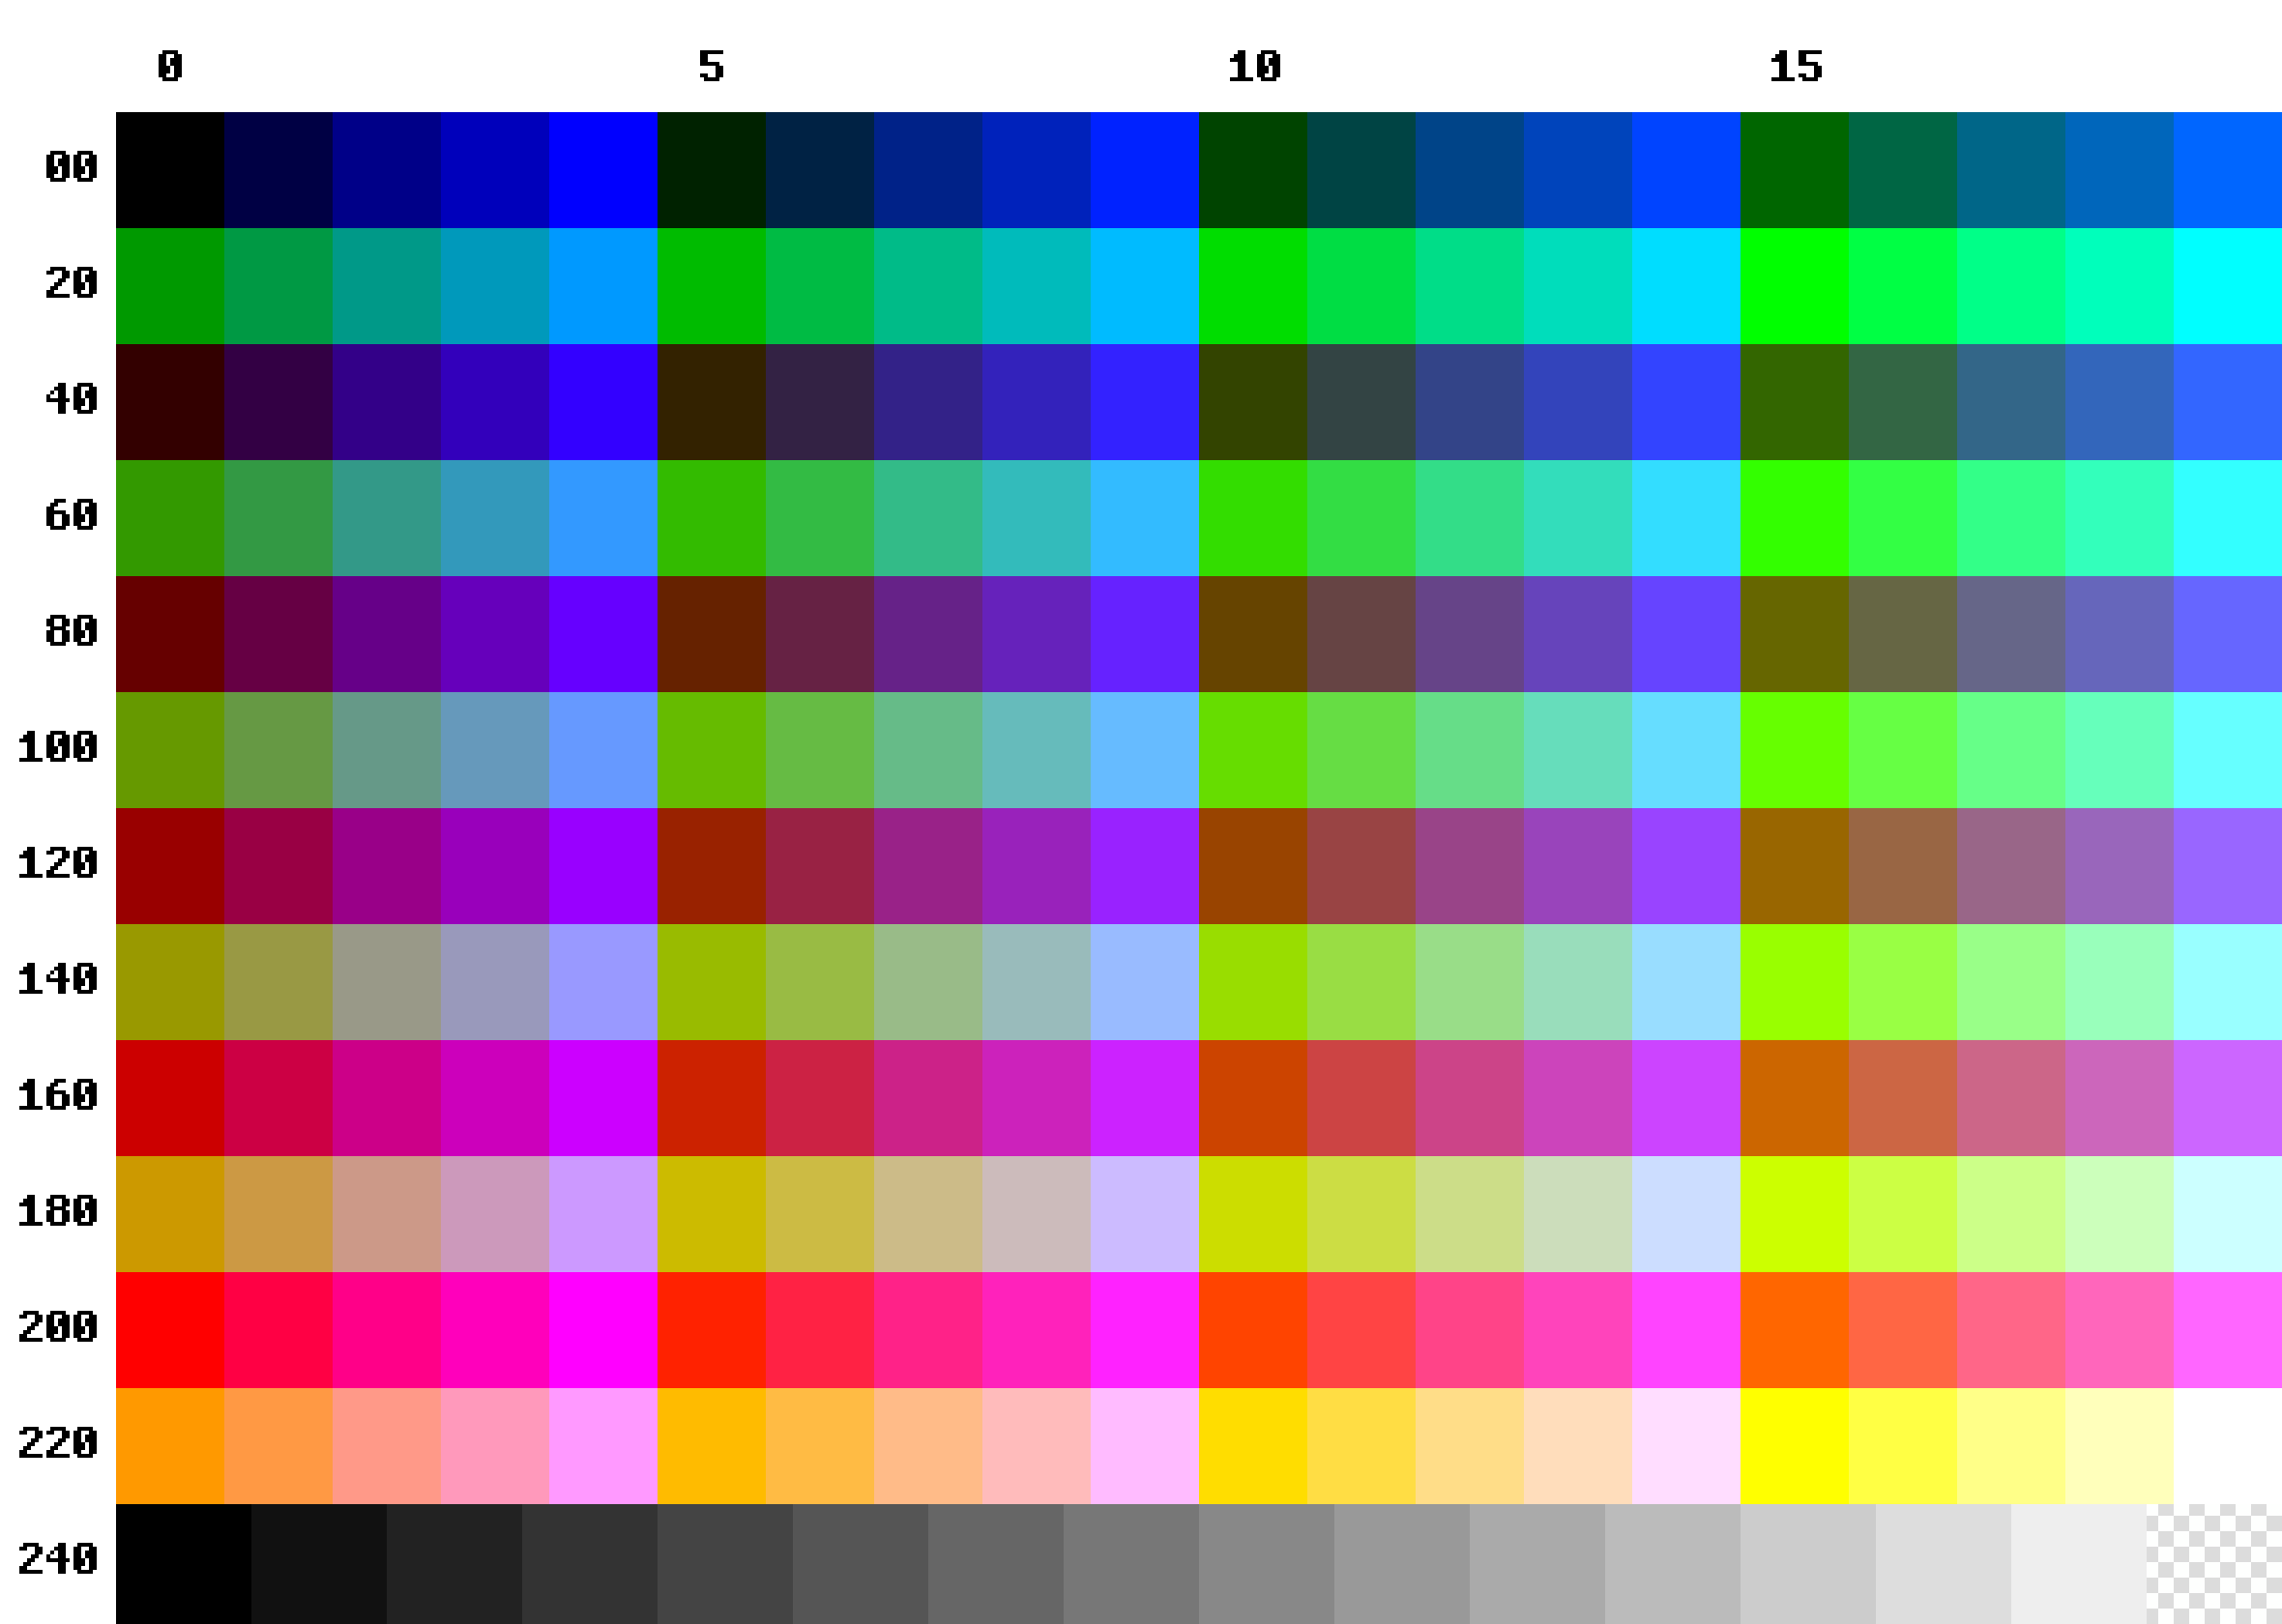
\includegraphics[width=\linewidth]{tsvmpal.png}
\captionof{figure}{\thismachine\ Colour Palette}
\label{fig:colourpalette}
}

{\centering
\fontsize{7pt}{0pt} % second argument is baselineskip but it's useless in table
\newlength{\extrarowheighttwo}
\setlength{\extrarowheighttwo}{\extrarowheight}
\setlength{\extrarowheight}{-0.4ex}

\begin{longtable}{*{2}{m{\textwidth}}}\hline
\endfirsthead
\endhead

\endfoot
\hline
\endlastfoot
\centering
\begin{tabulary}{\textwidth}{rl}
{\ttfamily 0} & {\ttfamily \#000F} \\
{\ttfamily 1} & {\ttfamily \#004F} \\
{\ttfamily 2} & {\ttfamily \#008F} \\
{\ttfamily 3} & {\ttfamily \#00BF} \\
{\ttfamily 4} & {\ttfamily \#00FF} \\
{\ttfamily 5} & {\ttfamily \#020F} \\
{\ttfamily 6} & {\ttfamily \#024F} \\
{\ttfamily 7} & {\ttfamily \#028F} \\
{\ttfamily 8} & {\ttfamily \#02BF} \\
{\ttfamily 9} & {\ttfamily \#02FF} \\
{\ttfamily 10} & {\ttfamily \#040F} \\
{\ttfamily 11} & {\ttfamily \#044F} \\
{\ttfamily 12} & {\ttfamily \#048F} \\
{\ttfamily 13} & {\ttfamily \#04BF} \\
{\ttfamily 14} & {\ttfamily \#04FF} \\
{\ttfamily 15} & {\ttfamily \#060F} \\
{\ttfamily 16} & {\ttfamily \#064F} \\
{\ttfamily 17} & {\ttfamily \#068F} \\
{\ttfamily 18} & {\ttfamily \#06BF} \\
{\ttfamily 19} & {\ttfamily \#06FF} \\
{\ttfamily 20} & {\ttfamily \#090F} \\
{\ttfamily 21} & {\ttfamily \#094F} \\
{\ttfamily 22} & {\ttfamily \#098F} \\
{\ttfamily 23} & {\ttfamily \#09BF} \\
{\ttfamily 24} & {\ttfamily \#09FF} \\
{\ttfamily 25} & {\ttfamily \#0B0F} \\
{\ttfamily 26} & {\ttfamily \#0B4F} \\
{\ttfamily 27} & {\ttfamily \#0B8F} \\
{\ttfamily 28} & {\ttfamily \#0BBF} \\
{\ttfamily 29} & {\ttfamily \#0BFF} \\
{\ttfamily 30} & {\ttfamily \#0D0F} \\
{\ttfamily 31} & {\ttfamily \#0D4F} \\
{\ttfamily 32} & {\ttfamily \#0D8F} \\
{\ttfamily 33} & {\ttfamily \#0DBF} \\
{\ttfamily 34} & {\ttfamily \#0DFF} \\
{\ttfamily 35} & {\ttfamily \#0F0F} \\
{\ttfamily 36} & {\ttfamily \#0F4F} \\
{\ttfamily 37} & {\ttfamily \#0F8F} \\
{\ttfamily 38} & {\ttfamily \#0FBF} \\
{\ttfamily 39} & {\ttfamily \#0FFF} \\
{\ttfamily 40} & {\ttfamily \#300F} \\
{\ttfamily 41} & {\ttfamily \#304F} \\
{\ttfamily 42} & {\ttfamily \#308F} \\
\end{tabulary}
\begin{tabulary}{\textwidth}{|rl}
{\ttfamily 43} & {\ttfamily \#30BF} \\
{\ttfamily 44} & {\ttfamily \#30FF} \\
{\ttfamily 45} & {\ttfamily \#320F} \\
{\ttfamily 46} & {\ttfamily \#324F} \\
{\ttfamily 47} & {\ttfamily \#328F} \\
{\ttfamily 48} & {\ttfamily \#32BF} \\
{\ttfamily 49} & {\ttfamily \#32FF} \\
{\ttfamily 50} & {\ttfamily \#340F} \\
{\ttfamily 51} & {\ttfamily \#344F} \\
{\ttfamily 52} & {\ttfamily \#348F} \\
{\ttfamily 53} & {\ttfamily \#34BF} \\
{\ttfamily 54} & {\ttfamily \#34FF} \\
{\ttfamily 55} & {\ttfamily \#360F} \\
{\ttfamily 56} & {\ttfamily \#364F} \\
{\ttfamily 57} & {\ttfamily \#368F} \\
{\ttfamily 58} & {\ttfamily \#36BF} \\
{\ttfamily 59} & {\ttfamily \#36FF} \\
{\ttfamily 60} & {\ttfamily \#390F} \\
{\ttfamily 61} & {\ttfamily \#394F} \\
{\ttfamily 62} & {\ttfamily \#398F} \\
{\ttfamily 63} & {\ttfamily \#39BF} \\
{\ttfamily 64} & {\ttfamily \#39FF} \\
{\ttfamily 65} & {\ttfamily \#3B0F} \\
{\ttfamily 66} & {\ttfamily \#3B4F} \\
{\ttfamily 67} & {\ttfamily \#3B8F} \\
{\ttfamily 68} & {\ttfamily \#3BBF} \\
{\ttfamily 69} & {\ttfamily \#3BFF} \\
{\ttfamily 70} & {\ttfamily \#3D0F} \\
{\ttfamily 71} & {\ttfamily \#3D4F} \\
{\ttfamily 72} & {\ttfamily \#3D8F} \\
{\ttfamily 73} & {\ttfamily \#3DBF} \\
{\ttfamily 74} & {\ttfamily \#3DFF} \\
{\ttfamily 75} & {\ttfamily \#3F0F} \\
{\ttfamily 76} & {\ttfamily \#3F4F} \\
{\ttfamily 77} & {\ttfamily \#3F8F} \\
{\ttfamily 78} & {\ttfamily \#3FBF} \\
{\ttfamily 79} & {\ttfamily \#3FFF} \\
{\ttfamily 80} & {\ttfamily \#600F} \\
{\ttfamily 81} & {\ttfamily \#604F} \\
{\ttfamily 82} & {\ttfamily \#608F} \\
{\ttfamily 83} & {\ttfamily \#60BF} \\
{\ttfamily 84} & {\ttfamily \#60FF} \\
{\ttfamily 85} & {\ttfamily \#620F} \\
\end{tabulary}
\begin{tabulary}{\textwidth}{|rl}
{\ttfamily 86} & {\ttfamily \#624F} \\
{\ttfamily 87} & {\ttfamily \#628F} \\
{\ttfamily 88} & {\ttfamily \#62BF} \\
{\ttfamily 89} & {\ttfamily \#62FF} \\
{\ttfamily 90} & {\ttfamily \#640F} \\
{\ttfamily 91} & {\ttfamily \#644F} \\
{\ttfamily 92} & {\ttfamily \#648F} \\
{\ttfamily 93} & {\ttfamily \#64BF} \\
{\ttfamily 94} & {\ttfamily \#64FF} \\
{\ttfamily 95} & {\ttfamily \#660F} \\
{\ttfamily 96} & {\ttfamily \#664F} \\
{\ttfamily 97} & {\ttfamily \#668F} \\
{\ttfamily 98} & {\ttfamily \#66BF} \\
{\ttfamily 99} & {\ttfamily \#66FF} \\
{\ttfamily 100} & {\ttfamily \#690F} \\
{\ttfamily 101} & {\ttfamily \#694F} \\
{\ttfamily 102} & {\ttfamily \#698F} \\
{\ttfamily 103} & {\ttfamily \#69BF} \\
{\ttfamily 104} & {\ttfamily \#69FF} \\
{\ttfamily 105} & {\ttfamily \#6B0F} \\
{\ttfamily 106} & {\ttfamily \#6B4F} \\
{\ttfamily 107} & {\ttfamily \#6B8F} \\
{\ttfamily 108} & {\ttfamily \#6BBF} \\
{\ttfamily 109} & {\ttfamily \#6BFF} \\
{\ttfamily 110} & {\ttfamily \#6D0F} \\
{\ttfamily 111} & {\ttfamily \#6D4F} \\
{\ttfamily 112} & {\ttfamily \#6D8F} \\
{\ttfamily 113} & {\ttfamily \#6DBF} \\
{\ttfamily 114} & {\ttfamily \#6DFF} \\
{\ttfamily 115} & {\ttfamily \#6F0F} \\
{\ttfamily 116} & {\ttfamily \#6F4F} \\
{\ttfamily 117} & {\ttfamily \#6F8F} \\
{\ttfamily 118} & {\ttfamily \#6FBF} \\
{\ttfamily 119} & {\ttfamily \#6FFF} \\
{\ttfamily 120} & {\ttfamily \#900F} \\
{\ttfamily 121} & {\ttfamily \#904F} \\
{\ttfamily 122} & {\ttfamily \#908F} \\
{\ttfamily 123} & {\ttfamily \#90BF} \\
{\ttfamily 124} & {\ttfamily \#90FF} \\
{\ttfamily 125} & {\ttfamily \#920F} \\
{\ttfamily 126} & {\ttfamily \#924F} \\
{\ttfamily 127} & {\ttfamily \#928F} \\
{\ttfamily 128} & {\ttfamily \#92BF} \\
\end{tabulary}
\begin{tabulary}{\textwidth}{|rl}
{\ttfamily 129} & {\ttfamily \#92FF} \\
{\ttfamily 130} & {\ttfamily \#940F} \\
{\ttfamily 131} & {\ttfamily \#944F} \\
{\ttfamily 132} & {\ttfamily \#948F} \\
{\ttfamily 133} & {\ttfamily \#94BF} \\
{\ttfamily 134} & {\ttfamily \#94FF} \\
{\ttfamily 135} & {\ttfamily \#960F} \\
{\ttfamily 136} & {\ttfamily \#964F} \\
{\ttfamily 137} & {\ttfamily \#968F} \\
{\ttfamily 138} & {\ttfamily \#96BF} \\
{\ttfamily 139} & {\ttfamily \#96FF} \\
{\ttfamily 140} & {\ttfamily \#990F} \\
{\ttfamily 141} & {\ttfamily \#994F} \\
{\ttfamily 142} & {\ttfamily \#998F} \\
{\ttfamily 143} & {\ttfamily \#99BF} \\
{\ttfamily 144} & {\ttfamily \#99FF} \\
{\ttfamily 145} & {\ttfamily \#9B0F} \\
{\ttfamily 146} & {\ttfamily \#9B4F} \\
{\ttfamily 147} & {\ttfamily \#9B8F} \\
{\ttfamily 148} & {\ttfamily \#9BBF} \\
{\ttfamily 149} & {\ttfamily \#9BFF} \\
{\ttfamily 150} & {\ttfamily \#9D0F} \\
{\ttfamily 151} & {\ttfamily \#9D4F} \\
{\ttfamily 152} & {\ttfamily \#9D8F} \\
{\ttfamily 153} & {\ttfamily \#9DBF} \\
{\ttfamily 154} & {\ttfamily \#9DFF} \\
{\ttfamily 155} & {\ttfamily \#9F0F} \\
{\ttfamily 156} & {\ttfamily \#9F4F} \\
{\ttfamily 157} & {\ttfamily \#9F8F} \\
{\ttfamily 158} & {\ttfamily \#9FBF} \\
{\ttfamily 159} & {\ttfamily \#9FFF} \\
{\ttfamily 160} & {\ttfamily \#C00F} \\
{\ttfamily 161} & {\ttfamily \#C04F} \\
{\ttfamily 162} & {\ttfamily \#C08F} \\
{\ttfamily 163} & {\ttfamily \#C0BF} \\
{\ttfamily 164} & {\ttfamily \#C0FF} \\
{\ttfamily 165} & {\ttfamily \#C20F} \\
{\ttfamily 166} & {\ttfamily \#C24F} \\
{\ttfamily 167} & {\ttfamily \#C28F} \\
{\ttfamily 168} & {\ttfamily \#C2BF} \\
{\ttfamily 169} & {\ttfamily \#C2FF} \\
{\ttfamily 170} & {\ttfamily \#C40F} \\
{\ttfamily 171} & {\ttfamily \#C44F} \\
\end{tabulary}
\begin{tabulary}{\textwidth}{|rl}
{\ttfamily 172} & {\ttfamily \#C48F} \\
{\ttfamily 173} & {\ttfamily \#C4BF} \\
{\ttfamily 174} & {\ttfamily \#C4FF} \\
{\ttfamily 175} & {\ttfamily \#C60F} \\
{\ttfamily 176} & {\ttfamily \#C64F} \\
{\ttfamily 177} & {\ttfamily \#C68F} \\
{\ttfamily 178} & {\ttfamily \#C6BF} \\
{\ttfamily 179} & {\ttfamily \#C6FF} \\
{\ttfamily 180} & {\ttfamily \#C90F} \\
{\ttfamily 181} & {\ttfamily \#C94F} \\
{\ttfamily 182} & {\ttfamily \#C98F} \\
{\ttfamily 183} & {\ttfamily \#C9BF} \\
{\ttfamily 184} & {\ttfamily \#C9FF} \\
{\ttfamily 185} & {\ttfamily \#CB0F} \\
{\ttfamily 186} & {\ttfamily \#CB4F} \\
{\ttfamily 187} & {\ttfamily \#CB8F} \\
{\ttfamily 188} & {\ttfamily \#CBBF} \\
{\ttfamily 189} & {\ttfamily \#CBFF} \\
{\ttfamily 190} & {\ttfamily \#CD0F} \\
{\ttfamily 191} & {\ttfamily \#CD4F} \\
{\ttfamily 192} & {\ttfamily \#CD8F} \\
{\ttfamily 193} & {\ttfamily \#CDBF} \\
{\ttfamily 194} & {\ttfamily \#CDFF} \\
{\ttfamily 195} & {\ttfamily \#CF0F} \\
{\ttfamily 196} & {\ttfamily \#CF4F} \\
{\ttfamily 197} & {\ttfamily \#CF8F} \\
{\ttfamily 198} & {\ttfamily \#CFBF} \\
{\ttfamily 199} & {\ttfamily \#CFFF} \\
{\ttfamily 200} & {\ttfamily \#F00F} \\
{\ttfamily 201} & {\ttfamily \#F04F} \\
{\ttfamily 202} & {\ttfamily \#F08F} \\
{\ttfamily 203} & {\ttfamily \#F0BF} \\
{\ttfamily 204} & {\ttfamily \#F0FF} \\
{\ttfamily 205} & {\ttfamily \#F20F} \\
{\ttfamily 206} & {\ttfamily \#F24F} \\
{\ttfamily 207} & {\ttfamily \#F28F} \\
{\ttfamily 208} & {\ttfamily \#F2BF} \\
{\ttfamily 209} & {\ttfamily \#F2FF} \\
{\ttfamily 210} & {\ttfamily \#F40F} \\
{\ttfamily 211} & {\ttfamily \#F44F} \\
{\ttfamily 212} & {\ttfamily \#F48F} \\
{\ttfamily 213} & {\ttfamily \#F4BF} \\
{\ttfamily 214} & {\ttfamily \#F4FF} \\
\end{tabulary}
\begin{tabulary}{\textwidth}{|rl}
{\ttfamily 215} & {\ttfamily \#F60F} \\
{\ttfamily 216} & {\ttfamily \#F64F} \\
{\ttfamily 217} & {\ttfamily \#F68F} \\
{\ttfamily 218} & {\ttfamily \#F6BF} \\
{\ttfamily 219} & {\ttfamily \#F6FF} \\
{\ttfamily 220} & {\ttfamily \#F90F} \\
{\ttfamily 221} & {\ttfamily \#F94F} \\
{\ttfamily 222} & {\ttfamily \#F98F} \\
{\ttfamily 223} & {\ttfamily \#F9BF} \\
{\ttfamily 224} & {\ttfamily \#F9FF} \\
{\ttfamily 225} & {\ttfamily \#FB0F} \\
{\ttfamily 226} & {\ttfamily \#FB4F} \\
{\ttfamily 227} & {\ttfamily \#FB8F} \\
{\ttfamily 228} & {\ttfamily \#FBBF} \\
{\ttfamily 229} & {\ttfamily \#FBFF} \\
{\ttfamily 230} & {\ttfamily \#FD0F} \\
{\ttfamily 231} & {\ttfamily \#FD4F} \\
{\ttfamily 232} & {\ttfamily \#FD8F} \\
{\ttfamily 233} & {\ttfamily \#FDBF} \\
{\ttfamily 234} & {\ttfamily \#FDFF} \\
{\ttfamily 235} & {\ttfamily \#FF0F} \\
{\ttfamily 236} & {\ttfamily \#FF4F} \\
{\ttfamily 237} & {\ttfamily \#FF8F} \\
{\ttfamily 238} & {\ttfamily \#FFBF} \\
{\ttfamily 239} & {\ttfamily \#FFFF} \\
{\ttfamily 240} & {\ttfamily \#000F} \\
{\ttfamily 241} & {\ttfamily \#111F} \\
{\ttfamily 242} & {\ttfamily \#222F} \\
{\ttfamily 243} & {\ttfamily \#333F} \\
{\ttfamily 244} & {\ttfamily \#444F} \\
{\ttfamily 245} & {\ttfamily \#555F} \\
{\ttfamily 246} & {\ttfamily \#666F} \\
{\ttfamily 247} & {\ttfamily \#777F} \\
{\ttfamily 248} & {\ttfamily \#888F} \\
{\ttfamily 249} & {\ttfamily \#999F} \\
{\ttfamily 250} & {\ttfamily \#AAAF} \\
{\ttfamily 251} & {\ttfamily \#BBBF} \\
{\ttfamily 252} & {\ttfamily \#CCCF} \\
{\ttfamily 253} & {\ttfamily \#DDDF} \\
{\ttfamily 254} & {\ttfamily \#EEEF} \\
{\ttfamily 255} & {\ttfamily \#0000} \\
\, & \, \\
\, & \, \\
\end{tabulary}
\end{longtable}

\captionof{table}{Index--RGBA Table of the Colour Palette}
}

\setlength{\extrarowheight}{\extrarowheighttwo}

\section{The Graphics Library}

\index{graphics (library)}Graphics library provides basic functions to communicate and manipulate the graphics adapter.

\namespaceis{Graphics}{graphics}

\begin{outline}
\1\formalsynopsis{TODO}{to be added.}
\end{outline}


\section{Graphics Memory Mapping}

\index{graphics memory mapping}

\begin{tabulary}{\textwidth}{rL}
Address & Description \\
\hline
-1048577..-1299456 & Screen Buffer \\
-1299457 & Screen Background RED \\
-1299458 & Screen Background GREEN \\
-1299459 & Screen Background BLUE \\
-1299460 & Command \\
-1299461..-1299472 & Command Arguments \\
-1299473..-1299474 & Screen Buffer Scroll Offset X \\
-1299475..-1299476 & Screen Buffer Scroll Offset Y \\
-1302527..-1302528 & Text Cursor Position in $row \times 80 + col$, stored in Little Endian \\
-1302529..-1305088 & Text Foreground Colours \\
-1305089..-1307648 & Text Background Colours \\
-1307649..-1310208 & Text Buffer \\
-1310209..-1310720 & Palettes in This Pattern: {\ttfamily 0b RRRR GGGG; 0b BBBB AAAA} \\
\end{tabulary}


\part{\thedos}
\chapter{\thedos}

\thedos\ is a Disk Operating System (usually) bundled with the distribution of the \thismachine.

All \thedos-related features requires the DOS to be fully loaded.




\chapter{Bootstrapping}

\index{boot process}\thedos\ goes through follwing progress to deliver the \code{A:/} prompt:

\section{Probing Bootable Devices}
BIOS

\section{The Bootloader}
LOADBOOT

Then the Bootsector will try to read and execute \code{A:/tvdos/TVDOS.SYS}

\section{TVDOS.SYS}
\thedos.SYS will load system libraries and variables and then will try to run the boot script by executing \code{A:/AUTOEXEC.BAT}

\section{AUTOEXEC.BAT}

AUTOEXEC can setup user-specific variables (e.g. keyboard layout) and launch the command shell of your choice, \code{COMMAND} is the most common shell.

Variables can be set or changed using \textbf{SET} commands.



\chapter{DOS Commands}

\index{commands (DOS)}\index{coreutils (DOS)}DOS commands are only valid under the DOS environment.

\begin{outline}
\1\dossynopsis{cat}{file}{Reads a file and pipes its contents to the pipe, or to the console if no pipes are specified.}
\1\dossynopsis{cd}{dir}{Change the current working directory. Alias: chdir}
\1\dossynopsis{cls}{Clears the text buffer and the framebuffer if available.}
\1\dossynopsis{cp}{from to}{Make copies of the specified file. The source file must not be a directory. Alias: copy}
\1\dossynopsis{date}{Prints the system date. Alias: time}
\1\dossynopsis{dir}{path}{Lists the contents of the specifed path, or the current working directory if no arguments were given. Alias: ls}
\1\dossynopsis{del}{file}{Deletes the file. Aliases: erase, rm}
\1\dossynopsis{echo}{text}{Print the given text or a variable.}
\1\dossynopsis{exit}{Exits the current command processor.}
\1\dossynopsis{mkdir}{path}{Creates a directory. Aliase: md}
\1\dossynopsis{rem}{Comment-out the line.}
\1\dossynopsis{set}{key=value}{Sets the global variable \code{key} to \code{value}, or displays the list of global variables if no arguments were given.}
\1\dossynopsis{ver}{Prints the version of \thedos.}
\end{outline}



\chapter{Using DOS Utils on JS}

DOS coreutils and some of the internal functions can be used on Javascript program.

To invoke the coreutils, use \code{\_G.shell.coreutils.*}

\begin{outline}
\1\inlinesynopsis[\_G.shell]{resolvePathInput}{path}{Returns fully-qualified path of the input path, relative to the current working directory.}
\1\inlinesynopsis[\_G.shell]{getPwdString}{}{Returns the current working directory as a string.}
\1\inlinesynopsis[\_G.shell]{getCurrentDrive}{}{Returns the drive letter of the current working drive.}
\1\inlinesynopsis[\_G.shell]{execute}{command}{Executes the DOS command.}
\end{outline}



\chapter{Pipes}

\index{pipe (DOS)}Pipe is a way to chain the IO of the one program/command into the different programs/commands in series.

A pipe can be either named or anonymous: named pipes are ones that are created by the user while the anonymous pipes are created by the DOS process as a result of the command pipelining.

\section{Command Pipelining}

In \thedos, a pipe can be used to route the output of a command into the other command. For example, \code{dir | less} will route the output of the \code{dir} into the text viewer called \code{less} so that the user can take their time examining the list of files in the directory, even if the list is taller that the terminal's height.

\section{User-defined Pipe}

A user program can create and interact with the pipe so long as it's \emph{named}. The contents of the pipe can be read and modified just like a Javascript variable.

Named pipes can be retrieved on \code{\_G.shell.pipes.*}

\section{Pipe-related Functions}

\begin{outline}
\1\inlinesynopsis[\_G.shell]{getPipe}{}{Returns the currently opened pipe. \code{undefined} is returned if no pipes are opened.}
\1\inlinesynopsis[\_G.shell]{appendToCurrentPipe}{text}{Appends the given text to the current pipe.}
\1\inlinesynopsis[\_G.shell]{pushAnonPipe}{contents}{Pushes an anonymous pipe to the current pipe stack.}
\1\inlinesynopsis[\_G.shell]{pushPipe}{pipeName, contents}{Pushes the pipe of given name to the current pipe stack.}
\1\inlinesynopsis[\_G.shell]{hasPipe}{}{Returns true if there is a pipe currently opened.}
\1\inlinesynopsis[\_G.shell]{removePipe}{}{Destroys the currently opened pipe and returns it. Any pipes on the pipe stack will be shifted down to become the next current pipe.}
\end{outline}


\chapter{File I/O}
\index{filesystem (DOS)}In \thedos, drives are assigned with a drive letter, and the drive currently booted on is always drive \textbf{A}.


\section{The File Descriptor}
\index{file descriptor (DOS)}A file is virtualised through the \emph{file descriptor} which provides the functions to manipulate the file. Do note that when a file descriptor is created, the file is not yet opened by the drive.

To create a file descriptor, use the provided function \code{files.open(fullPath)}. \code{fullPath} is a fully qualified path of the file that includes the drive letter.

\section{Manipulating a File}
A file has folliwing properties and can be manipulated using following functions:

Properties:

\begin{outline}
\1\propertysynopsis{size}{Int}{Returns a size of the file in bytes.}
\1\propertysynopsis{path}{String}{Returns a path (NOT including the drive letter) of the file. Paths are separated using reverse solidus.}
\1\propertysynopsis{fullPath}{String}{Returns a fully qualified path (including the drive letter) of the file. Paths are separated using reverse solidus.}
\1\propertysynopsis{driverID}{String}{Returns a filesystem driver ID associated with the file.}
\1\propertysynopsis{driver}{[Object object]}{Returns a filesystem driver (a Javascript object) for the file.}
\1\propertysynopsis{isDirectory}{Boolean}{Returns true if the path is a directory.}
\1\propertysynopsis{name}{String}{Returns the name part of the file's path.}
\1\propertysynopsis{parentPath}{String}{Returns a parent path of the file.}
\1\propertysynopsis{exists}{Boolean}{Returns true if the file exists on the device.}
\end{outline}

Functions:

\begin{outline}
\1\formalsynopsis{pread}{pointer: Int, count: Int, offset: Int}{Reads the file bytewise and puts it to the memory starting from the pointer.}
 \2\argsynopsis{count}{how many bytes to read}
 \2\argsynopsis{offset}{when reading a file, how many bytes to skip initially}
\1\formalsynopsis{bread}{}[Array]{Reads the file bytewise and returns the content in Javascript array.}
\1\formalsynopsis{sread}{}[String]{Reads the file textwise and returns the content in Javascript string.}
\1\formalsynopsis{pwrite}{pointer: Int, count: Int, offset: Int}
{Writes the bytes stored in the memory starting from the pointer to file.}
 \2\argsynopsis{count}{how many bytes to write}
 \2\argsynopsis{offset}{when writing to the file, how many bytes on the file to skip before writing a first byte.}
\1\formalsynopsis{bwrite}{bytes: UintArray}{Writes the bytes to the file.}
\1\formalsynopsis{swrite}{string: String}{Writes the string to the file.}
\1\formalsynopsis{flush}{}{Flush the contents on the write buffer to the file immediately. Will do nothing if there is no write buffer implemented --- a write operation will always be performed imemdiately in such cases.}
\1\formalsynopsis{close}{}{Tells the underlying device (usually a disk drive) to close a file. When dealing with multiple files on a single disk drive (of which can only have a single active---or opened---file), the underlying filesystem driver will automatically swap the files around, so this function is normally unused.}
\1\formalsynopsis{list}{}[Array or undefined]{Lists files inside of the directory. If the path is indeed a directory, an array of file descriptors will be returned; \code{undefined} otherwise.}
\1\formalsynopsis{touch}{}[Boolean]{Updates the file's access time if the file exists; a new file will be created otherwise. Returns true if successful.}
\1\formalsynopsis{mkDir}{}[Boolean]{Creates a directory to the path. Returns true if successful.}
\1\formalsynopsis{mkFile}{}[Boolean]{Creates a new file to the path. Returns true if successful.}
\1\formalsynopsis{remove}{}[Boolean]{Removes a file. Returns true if successful.}
\end{outline}


\section{The Device Files}

\index{device file}Some devices are also virtualised through the file descriptor, and they are given a special path. (their fullPath does not contain a drive letter)

\begin{outline}
\1\inlinesynopsis{RND}{returns random bytes upon reading}
 \2\argsynopsis{pread}{returns the specified number of random bytes}
\1\inlinesynopsis{NUL}{returns EOF upon reading}
 \2\argsynopsis{pread}{returns the specified number of EOFs}
 \2\argsynopsis{bread}{returns an empty array}
 \2\argsynopsis{sread}{returns an empty string}
\1\inlinesynopsis{ZERO}{returns zero upon reading}
 \2\argsynopsis{pread}{returns the specified number of zeros}
\1\inlinesynopsis{CON}{manipulates the screen text buffer, disregarding the colours}
 \2\argsynopsis{pread}{reads the texts as bytes.}
 \2\argsynopsis{bread}{reads the texts as bytes.}
 \2\argsynopsis{sread}{reads the texts as a string.}
 \2\argsynopsis{pwrite}{writes the bytes from the given pointer.}
 \2\argsynopsis{bwrite}{identical to \code{print()} except the given byte array will be casted to string.}
 \2\argsynopsis{swrite}{identical to \code{print()}.}
\1\inlinesynopsis{FBIPF}{decodes IPF-formatted image to the framebuffer. Use the \emph{Graphics} library for the encoding.}
 \2\argsynopsis{pwrite, bwrite}{decodes the given IPF binary data. Offsets and counts for \code{pwrite} are ignored.}
\end{outline}


\chapter{DOS Libraries}


\section{Input}

\dosnamespaceis{Input}{input}

\begin{outline}
\1\inlinesynopsis{changeKeyLayout}{layoutName}{Changes the key layout. The key layout file must be stored as \code{A:/tvdos/layoutName.key}}
\1\inlinesynopsis{withEvent}{callback}{Invokes the callback function when an input event is available.}
\end{outline}

\subsection{Input Events}

Input events are Javascript array of: $$ [\mathrm{event\ name,\ arg_1,\ arg_2 \cdots arg_n}] $$, where:

\begin{outline}
\1event name --- one of following: \textbf{key\_down}, \textbf{mouse\_down}, \textbf{mouse\_move}
\1arguments for \textbf{key\_down}:
 \2\argsynopsis{\argN{1}}{Key Symbol (string) of the head key}
 \2\argsynopsis{\argN{2}}{Repeat count of the key event}
 \2\argsynopsis{\argN{3}..\argN{10}}{The keycodes of the pressed keys}
\1arguments for \textbf{mouse\_down}:
 \2\argsynopsis{\argN{1}}{X-position of the mouse cursor}
 \2\argsynopsis{\argN{2}}{Y-position of the mouse cursor}
 \2\argsynopsis{\argN{3}}{Always the integer 1.}
\1arguments for \textbf{mouse\_move}:
 \2\argsynopsis{\argN{1}}{X-position of the mouse cursor}
 \2\argsynopsis{\argN{2}}{Y-position of the mouse cursor}
 \2\argsynopsis{\argN{3}}{1 if the mouse button is held down (i.e. dragging), 0 otherwise}
 \2\argsynopsis{\argN{4}}{X-position of the mouse cursor on the previous frame (previous V-blank of the screen)}
 \2\argsynopsis{\argN{5}}{Y-position of the mouse cursor on the previous frame}
\end{outline}

\section{GL}

\dosnamespaceis{Graphics}{gl}

\begin{outline}
\end{outline}


\part*{Bibliography}

\chapter*{Bibliography}
\begin{itemlist}
\item Song, Minjae. 2021. ``Terran BASIC Reference Manual for Language Version 1.2, Third Edition''.
\item Wikipedia. ``List of DOS commands.'' Updated 2022-08-29 15:00. \url{https://en.wikipedia.org/wiki/List_of_DOS_commands}.
\item Wikipedia. ``Pipeline (software).'' Updated 2022-07-17 06:21. \url{https://en.wikipedia.org/wiki/Pipeline_(software)}.
\end{itemlist}


{
\let\clearpage\relax
\chapter*{\ \\ Disclaimers}

\oreallypress{} is entirely fictional publishing entity; \oreallypress{} has no affiliation whatsoever with any of the real-world publishers.

% Level of humour used in this document is \emph{super-corny}. Do not use this atrocious humour for a purpose of real-world entertainment; we take no responsibility for the consequences---losing your friends, get shunned by people, etc.
}

\chapter*{Copyright}

The source code for \thismachine\ and this documentation are distributed under the following terms:

\copyright\ 2020-- \ Minjae Song (``CuriousTorvald'')

Permission is hereby granted, free of charge, to any person obtaining a copy
of this software and associated documentation files (the ``Software''), to deal
in the Software without restriction, including without limitation the rights
to use, copy, modify, merge, publish, distribute, sublicense, and/or sell
copies of the Software, and to permit persons to whom the Software is
furnished to do so, subject to the following conditions:

The above copyright notice and this permission notice shall be included in all
copies or substantial portions of the Software.

THE SOFTWARE IS PROVIDED ``AS IS'', WITHOUT WARRANTY OF ANY KIND, EXPRESS OR
IMPLIED, INCLUDING BUT NOT LIMITED TO THE WARRANTIES OF MERCHANTABILITY,
FITNESS FOR A PARTICULAR PURPOSE AND NONINFRINGEMENT. IN NO EVENT SHALL THE
AUTHORS OR COPYRIGHT HOLDERS BE LIABLE FOR ANY CLAIM, DAMAGES OR OTHER
LIABILITY, WHETHER IN AN ACTION OF CONTRACT, TORT OR OTHERWISE, ARISING FROM,
OUT OF OR IN CONNECTION WITH THE SOFTWARE OR THE USE OR OTHER DEALINGS IN THE
SOFTWARE.

\printindex

\afterpage{\pagestyle{empty}\null\newpage}

\end{document}
